\chapter{OWL}
\label{chap:owl}

Im letzten Kapitel wurde die Basis geschaffen um die eigentlich Ontologiesprache OWL zu analysieren. In diesem Kapitel, welches auf der W3C-Spezifikation~\cite{w3owl} basiert, wird diese nun genauer betrachtet. Bei OWL (Web Ontology Language) und OWL2 handelt es sich um die Ontologie-Sprache für das semantische Web, also um eine Sprache um Ontologien auszudrücken.~\cite{cambSemOWL} Wie RDF wurde auch OWL entwickelt um Informationen nicht nur anzuzeigen, sondern auch zu verarbeiten. Durch zusätzliches Vokabular, wie zum Beispiel Beziehungen zwischen Klassen, und erweiterte formale Semantik hat der Benutzer mehr Möglichkeiten als bei RDF oder auch XML.

\section{OWL Syntax}
\label{sec:owl_owl_syntax}
Auch für OWL stehen verschiedene Schreibweisen zur Verfügung, welche für verschiedene Anwendungszwecke gedacht sind:
\begin{itemize}
	\item \textit{RDF/XML Syntax für OWL}

        Entspricht RDF/XML Syntax mit einer speziellen Übersetzung für OWL-Konstrukte. Dabei handelt es sich um die einzige Syntax, welche von allen OWL2-Tools unterstützt wird.
	\item \textit{OWL/XML Syntax}

        XML Syntax für OWL.
	\item \textit{Functional-Style Syntax}

        Zur Vereinfachung der ursprünglichen Spezifikation; Unterstützt Grundlagen zur Implementation von OWL2 mittels APIs und Reasoners
	\item \textit{Turtle Syntax}

        Bei der Tutrtle Syntax handelt es sich um eine textuelle Syntax, welche die Beschreibung eines RDF-Graphen in kompakter und natürlicher Form erlaubt.

        \begin{lstlisting}[caption={Beispiel der Turtle Syntax\protected\footmark}]
            <#green-goblin>
                rel:enemyOf <#spiderman> ;
                a foaf:Person ;    # in the context of the Marvel universe
                foaf:name "Green Goblin".
        \end{lstlisting}
        \footnotetext{Beispiel von \url{http://www.w3.org/TR/turtle/#sec-intro}}
	\item \textit{Manchester Syntax}

        Vereinfacht das Lesen für nicht logikaffine Leser.
\end{itemize}

Dabei ist zu sagen, dass Werkzeuge existieren, welche eine Übersetzung zwischen den verschiedenen Schreibweisen vornehmen.

Bei OWL handelt es sich nicht um eine Schemasprache. Im Gegensatz zu XML beschreibt OWL nicht wie ein Dokument aufgebaut sein muss. So kann auch nicht vorgeschrieben werden, dass ein bestimmtes Element vorhanden sein muss.

\section{Wissen modellieren}
\label{sec:owl_owl_wissenModellieren}
Bei OWL handelt sich um eine wissensbasierte Repräsentationssprache. Sie bildet das Wissen einer Domäne ab. Es wird versucht, eine Domäne in OWL so abzubilden, dass das menschliche Wissen widerspiegelt wird. Dabei gibt es keine Möglichkeit sämtliche Aspekte des menschlichen Wissens abzubilden. OWL kann aber als mächtige Modellierungssprache bezeichnet werden. Das Ergebnis einer solchen Modellierung nennt man, wie bereits erwähnt, eine Ontologie.

Um das Abbilden von Wissen zu erklären, wird in den folgenden Abschnitten der grundsätzliche Aufbau von OWL beschrieben. Die grundlegenden Elemente sind Axiome, Entitäten und Ausdrücke (Expressions).

\begin{itemize}
	\item \textit{Axiom}

        Grundlegende Aussagen.

        Grundaussagen  oder Basispropositionen wie ``Abenteuerreisen sind Reisen'' werden in OWL Axiome genannt. Es handelt sich  um ``Stücke des Wissens'', welche je nach Sachlage wahr oder falsch sein können. Dies unterscheidet Axiome grundlegend von Entitäten und Ausdrücken.

    \item \textit{Entitäten}

        Elemente, welche konkrete Objekte aus der realen Welt abbilden.

        Grundbestandteile einer Aussage, wie zum Beispiel die Objekte \textit{Abenteuerreise} und \textit{Reise} oder die Beziehung \textit{sind}, werden allgemein Entitäten genannt. Konkrete Objekte werden dabei als Individuen (Individuals), Kategorien als Klassen und Beziehungen als Eigenschaften (Properties) bezeichnet. Beziehungen werden in ObjectProperties (Relation zwischen zwei Individuen), DataProperties (spezifischer Datenwert eines Objektes) und AnnotationProperties (zusätzliche Information zu einem Objekt) unterteilt.

	\item \textit{Expression (Ausdruck)}

        Ausdrücke sind Kombinationen aus Enitiäten, die es ermöglichen komplexe Beschreibungen aufzubauen.

        Entitäten können mithilfe eines Konstruktors kombiniert werden. Zum Beispiel \textit{Abenteuerreise} und die Klasse \textit{Reise}. Diese Vereinigung wird als so genannte Class Expression abgebildet und kann als neue Entität angesehen werden.

        \begin{lstlisting}[caption={Beispiel eines Ausdrucks}]
            EquivalentClasses(
                :Restaurant
                :Gaststätte
            )
        \end{lstlisting}

        Ausdrücke für Klassen sind sehr mächtig, Ausdrücke für Eigenschaften sind hingegen schwächer.
\end{itemize}

Ein Mensch kann Schlussfolgern. Er kann nachvollziehen, dass es Situationen gibt, bei welchen aus einer Tatsache eine nächste folgt. Wenn also eine Aussage wahr ist, folgt daraus, dass eine andere auch zutrifft. Dies wird mittels sogenannten Reasonern umgesetzt. Ein Reasoner kann also Konsequenzen ermitteln. Es kann schwierig zu verstehen sein, wie Axiome miteinander interagieren. Dieser Zusammenhang kann als Stärke und als Schwäche von OWL angesehen werden. Als Stärke, weil der Reasoner Informationen aufdeckt, welche ein Mensch ggf.\ nicht erkennen würde. Eine Schwäche hingegen, weil es schwer ist, die unmittelbare Wirkung vorherzusehen.

\section{Die wichtigsten Elemente von OWL}
\label{sec:owlRdf_owl_wichtigsteElemente}

\subsection{Klassen, Subklassen und Individuen}
\label{sec:owlRdf_owl_wissenModellieren_wichtigsteElemente_Classen}

\textbf{Klassen}

\textit{Ausflug} ist eine Klasse.

\begin{lstlisting}[caption={Beispiel einer Klasse}]
    <!-- http://www.semanticweb.org/sosterwalder/ontologies/2014/10/reiseplaner#Ausflug -->
    <owl:Class rdf:about="&reiseplaner;Ausflug"/>
\end{lstlisting}

\textbf{Subklassen}

\textit{Landgasthaus} ist Subklasse von \textit{Restaurant}.

\begin{lstlisting}[caption={Beispiel einer Subklasse}]
    <!-- http://www.semanticweb.org/sosterwalder/ontologies/2014/10/reiseplaner#Landgasthaus -->
    <owl:Class rdf:about="&reiseplaner;Landgasthaus">
        <rdfs:subClassOf rdf:resource="&reiseplaner;Restaurant"/>
    </owl:Class>
\end{lstlisting}
Subklassen werden nicht nur verwendet um Abhängigkeiten darzustellen, sondern auch um Klassenhierarchien zu modellieren. Mittels Subklassen werden also allgemeine Beziehungen der Klassen abgebildet, so zum Beispiel die Relation ``Ein Landgasthaus ist ein Restaurant.''

\textbf{Individuum}

\textit{Seilpark Balmberg} ist ein Individuum der Klasse \textit{Ausflug}. Individuuen können auch von mehreren Klassen gleichzeitig abstammen.

\begin{lstlisting}[caption={Beispiel eines Individuums}]
    <!-- http://www.semanticweb.org/sosterwalder/ontologies/2014/10/reiseplaner#Seilpark -->
    <owl:NamedIndividual rdf:about="&reiseplaner;Seilpark">
        <rdf:type rdf:resource="&reiseplaner;Ausflug"/>
        <reiseplaner:alter rdf:datatype="&xsd;integer">6</reiseplaner:alter>
        <reiseplaner:erfordert>mut</reiseplaner:erfordert>
        <reiseplaner:erfordert>geschicklichkeit</reiseplaner:erfordert>
        <reiseplaner:url>http://www.seilpark-balmberg.ch/</reiseplaner:url>
        <reiseplaner:hatStandort rdf:resource="&reiseplaner;Balmberg"/>
    </owl:NamedIndividual>
\end{lstlisting}

\newpage

Individuen können gleichgestellt werden oder sich auch gegenseitig ausschliessen.

\begin{lstlisting}[caption={Beispiel einer Gleichstellung von Individuen}]
    <!-- http://www.semanticweb.org/sosterwalder/ontologies/2014/10/reiseplaner#Seilpark -->
    <owl:NamedIndividual rdf:about="&reiseplaner;Seilpark">
        <rdf:type rdf:resource="&reiseplaner;Ausflug"/>
        ...
        <owl:sameAs rdf:resource="&reiseplaner;Seilpark_Balmberg"/>
    </owl:NamedIndividual>
\end{lstlisting}

\begin{lstlisting}[caption={Beispiel einer Differenzierung von Individuen}]
    <rdf:Description>
        <rdf:type rdf:resource="&owl;AllDifferent"/>
        <owl:distinctMembers rdf:parseType="Collection">
            <rdf:Description rdf:about="&reiseplaner;Seilpark"/>
            <rdf:Description rdf:about="&reiseplaner;Seilpark_Balmberg"/>
            <rdf:Description rdf:about="&reiseplaner;Seilpark_Pilatus"/>
        </owl:distinctMembers>
    </rdf:Description>

\end{lstlisting}



\subsubsection{Eigenschaften}
\label{subsubsec:owlRdf_owl_wissenModellieren_wichtigsteElemente_Propertys}

\textbf{Objekt-Eigenschaften (ObjectProperties)}

Hierbei handelt es sich um eine Beziehung zwischen zwei Individuen.

\begin{lstlisting}[caption={Beispiel einer Objekteigenschaft \textit{hatOrt} und deren Anwendung}]
    <owl:ObjectProperty rdf:about="&reiseplaner;hatOrt">
        <rdfs:range rdf:resource="&reiseplaner;Ort"/>
        <rdfs:domain rdf:resource="&reiseplaner;Region"/>
    </owl:ObjectProperty>
    ...
    
    <owl:Thing rdf:about="&reiseplaner;Bern">
        <rdf:type rdf:resource="&owl;NamedIndividual"/>
        <reiseplaner:distanzZuAusgangpunkt rdf:datatype="&xsd;integer">0</reiseplaner:distanzZuAusgangpunkt>
        <reiseplaner:hatOrt rdf:resource="&reiseplaner;Bern"/>
        <reiseplaner:hatOrt rdf:resource="&reiseplaner;Ersigen"/>
    </owl:Thing>
\end{lstlisting}

Dabei kann eingeschränkt werden auf welche und mit welcher Klasse einer Domäne eine Objekteigenschaft angewendet werden darf.

\begin{lstlisting}[caption={Beispiel von Einschränkungen der Objekteigenschaft \textit{hatRegion}}]
    <!-- http://www.semanticweb.org/sosterwalder/ontologies/2014/10/reiseplaner#hatRegion -->
    <owl:ObjectProperty rdf:about="&reiseplaner;hatRegion">
        <rdfs:domain rdf:resource="&reiseplaner;Land"/>
        <rdfs:range rdf:resource="&reiseplaner;Region"/>
    </owl:ObjectProperty>
\end{lstlisting}

\textbf{Subeigenschaften}
Es besteht die Möglichkeit Untereigenschaften zu definieren.

\begin{lstlisting}[caption={Beispiel der Objekteigenschaft \textit{hatGemeinde} als Subeigenschaft von \textit{hatRegion}}]
    <!-- http://www.semanticweb.org/sosterwalder/ontologies/2014/10/reiseplaner#hatGemeinde -->
    <owl:ObjectProperty rdf:about="&reiseplaner;hatGemeinde">
        <rdfs:subPropertyOf rdf:resource="&reiseplaner;hatRegion"/>
    </owl:ObjectProperty>
\end{lstlisting}

\textbf{Datentypen-Eigenschaften (DataProperties)}

Datentypen-Eigenschaften definieren und beschreiben einen spezifischen Datenwert eines Individuums. Dies kann beispielsweise das Alter oder die Grösse einer Person sein. Datentypen-Eigenschaft können frei definiert werden und, bei Bedarf, an vordefinierte Wertetypen gebunden werden. Eine Auflistung dieser befindet sich unter~\footnote{\url{http://www.w3.org/TR/owl2-syntax/#Datatype_Maps}}.

% Datentypen Eigenschaft: TODO: bei uns anwenden.\\
% \noindent\hspace*{15mm} <Person rdf:about="'John"'>\\
% \noindent\hspace*{25mm}   <hasAge rdf:datatype="http://www.w3.org/2001/XMLSchema\#integer"'>51</hasAge>\\
% \noindent\hspace*{15mm} </Person>\\

\begin{lstlisting}[caption={Beispiel der Datentypen-Eigenschaft \textit{anzahlTeilnehmer} und deren Anwendung bei einem Individuum}]
    <!-- http://www.semanticweb.org/sosterwalder/ontologies/2014/10/reiseplaner#anzahlTeilnehmer -->
    <owl:DatatypeProperty rdf:about="&reiseplaner;anzahlTeilnehmer">
        <rdfs:range rdf:resource="&xsd;integer"/>
        <rdfs:subPropertyOf rdf:resource="&owl;topDataProperty"/>
    </owl:DatatypeProperty>
    ...
    <!-- http://www.semanticweb.org/sosterwalder/ontologies/2014/10/reiseplaner#AdventureRooms -->
    <owl:NamedIndividual rdf:about="&reiseplaner;AdventureRooms">
        ...
        <reiseplaner:anzahlTeilnehmer rdf:datatype="&xsd;integer">12</reiseplaner:anzahlTeilnehmer>
        ...
    </owl:NamedIndividual>
\end{lstlisting}

\newpage

\section{Ontologien}
\label{sec:owl_owl_Ontologien}

Die gesamten Informationen zu einem Thema werden in Ontologien abgebildet. Diese können von verschiedenen Anwendungen genutzt werden.

\begin{lstlisting}[caption={Beispiel einer Definition einer Ontologie}]
    <owl:Ontology rdf:about="http://www.semanticweb.org/sosterwalder/ontologies/2014/10/reiseplaner"/>
\end{lstlisting}

Ontologien werden in bzw.\ als OWL-Dokumente abgespeichert. Diese können entweder rein lokal, oder aber im Internet zur Verfügung gestellt werden.
Beim Schreiben einer Ontologie können zusätzliche Namespaces verwendet werden, so zum Beispiel \textit{http://www.w3.org/2001/XMLSchema\#}. Ist ein Namespace z.B. nur per Internet verfügbar, so kann dieser beispielsweise bei einem Ausfall der Internetverbindung nicht genutzt werden. Daher sollte berücksichtigt werden, dass Namespaces kontrollierbar im Sinne der Verfügbarkeit sein sollten.

Informationen aus einer Ontologie können in einer anderen verwendet werden. Dazu muss diese allerdings importiert werden.

\begin{lstlisting}[caption={Beispiel eines Importes einer Ontologie}]
    <owl:Ontology rdf:about="http://example.com/owl/families\">
      <owl:imports rdf:resource="http://example.org/otherOntologies/families.owl" />
    </owl:Ontology>
\end{lstlisting}


Um bei der Verwendung von Objekten aus anderen Ontologien eine Umbenennung zu umgehen, kann direkt auf das entsprechende Objekt referenziert werden.

\begin{lstlisting}[caption={Beispiel einer Referenzierung auf ein Objekt einer externen Ontologie}]
    <owl:DatatypeProperty rdf:about="hasAge">
      <owl:equivalentProperty rdf:resource="\&otherOnt;age"/>
    </owl:DatatypeProperty>
\end{lstlisting}

\section{OWL Untersprachen}
\label{sec:owl_owl_Untersprachen}
OWL ist in drei Untersprachen aufgeteilt. Jede dieser Sprachen wurde für die Verwendung durch verschiedene Anwendergruppen entwickelt. Dabei handelt es sich um OWL Lite, OWL DL und OWL Full. Die neue Version OWL2 unterscheidet zusätzlich zwischen OWL2 QL, OWL2 EL und OWL2 RL.\ Dabei handelt es sich um weitere Unterklassen von OWL2 DL, welche wiederum eine Untersprache von OWL2 Full ist. Diese sollen hier nicht weiter analysiert werden. Genauere Informationen zu den einzelnen Untersprachen finden sich unter~\footnote{\url{http://www.w3.org/TR/2004/REC-owl-features-20040210/#s1.3}}, genauere Informationen zu den OWL2 Profilen finden sich unter~\footer{\url{http://www.w3.org/TR/owl2-profiles/}}.

\section{OWL-Werkzeuge}
\label{sec:owl_owl_OwlTools}
Es wird typischerweise zwischen zwei Arten von Ontologiewerkzeugen unterschieden. Der Editor, welcher für das Erzeugen und Ändern von Ontologien zuständig ist, und der Reasoner, welcher fähig ist logische Folgerungen aus dem bestehenden Wissen abzuleiten.

\noindent\rule[1ex]{\textwidth}{1pt}
\vspace{0.1pt}
\begin{wrapfigure}[5]{l}{0.1\textwidth}
    \vspace{-19pt}
    
\includegraphics[width=0.1\textwidth]{bilder/owl.png}
\end{wrapfigure}
Diese Sprachen mögen nützlich sein um Ontologien zu modellieren, sie sind aber in der Formulierung und vorallem zum Lesen eher umständlich. An diesem Punkt kommt der Editor ins Spiel. Mittels mehr oder weniger freundlichen Ontologiewerkzeugen lässt sich eine Ontologie intuitiv und übersichtlich abbilden. Wir haben in unserem Beispiel das in der Fachwelt weitverbreitete Werkzeug Protégé der Universität Stanford verwendet.


\begin{figure}[H]
\centering \rotatebox{0}{\scalebox{0.5}[0.5]{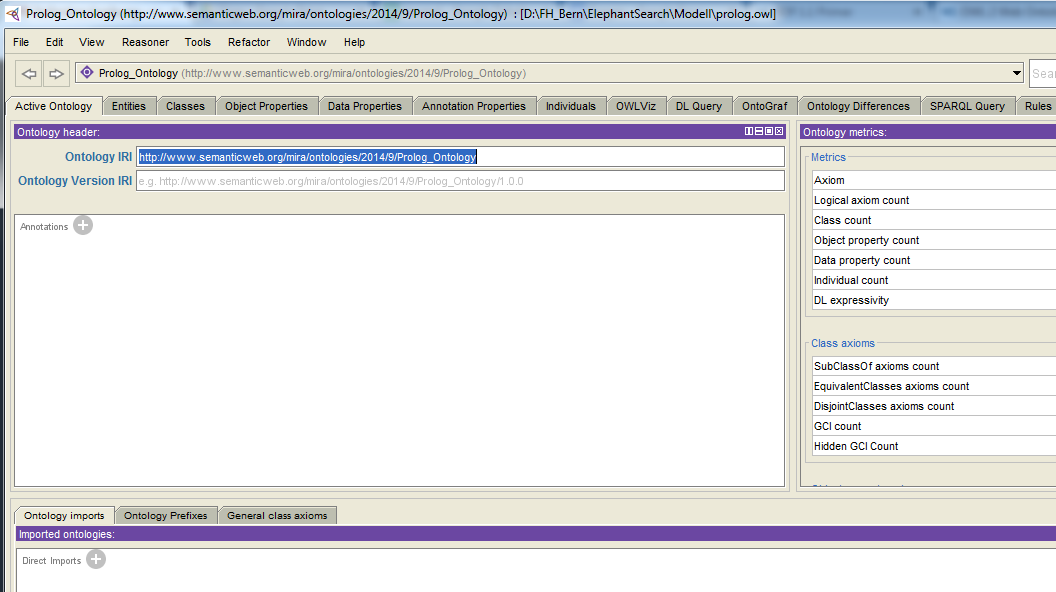
\includegraphics{bilder/protege.png}}}
\caption{Übersichtsfenster der Anwendung Protégé\label{fig:protege}\protect\footnotemark}
\end{figure}
\footnotetext{Eigens erstellter Screenshot von Protégé}


\vspace{0.1pt}
\noindent\rule[1ex]{\textwidth}{1pt}



% Quellen
% w3c
% http://www.w3.org/TR/2012/REC-owl2-primer-20121211/
% http://www.w3.org/2001/sw/wiki/OWL
% http://www.w3.org/TR/2014/NOTE-rdf11-primer-20140624/
